This introductory section lays the theoretical foundation of Bravais lattices and GNNs. 
We start with a short recap of lattice structures in two and three dimensions and then continue with 
the most fundamental background of Neural Networks (NNs) and Graph Neural Networks (GNNs).
Results on Bravais lattices can be found in many textbooks. Subsection~\ref{sec:brav_latt} follows \cite{Schwarzenberger} and \cite{symGroupsApplications}.
An introduction to NNs and GNNs can be found for example in \cite{bookNN1}, \cite{bookNN2} and in~\cite{IntroMessagePassing}
which are also the main reference for section~\ref{sec:intro_nn} and section~\ref{sec:fund_gnns}.

\subsection{Bravais Lattices}
\label{sec:brav_latt}
Let $d\in\N$ and $\{b_i\}_{i=1,\dots,d}\subset \R^d$ a basis of $\R^d$. The set 
\begin{equation*}
    \Omega\coloneq\left\{\sum_{i=1}^{d}z_i b_i: z_i\in\Z\,\forall i\in\{1,\dots,d\}\right\}
\end{equation*}
is called a $d$-dimensional lattice. Given any subset $S\subset\R^d$, we define its point group $G_S$ to be
\begin{equation*}
    G_S\coloneq \left\{M\in O(d) : MS=S\right\}\subset O(d).
\end{equation*}
$G_S$ is obviously a subgroup of $O(d)$. We say that two $d$-dimensional lattices $\Omega_1, \Omega_2\subset \R^d$ are of the same Bravais type if
there exists $g\in GL_n(\R)$ such that $G_{\Omega_1}=g G_{\Omega_2} g^{-1}$ and $\Omega_1=g\Omega_2$. 
Being of the same Bravais type introduces an equivalence relation on the set of all $d$-dimensional lattices. We refer to the equivalence classes as Bravais classes.
A natural question arising is about the total number of Bravais classes. Despite being a very interesting and challenging problem,
we will leave this question to the mathematicians. For us, the result is more important than the actual proof. One obtains the following result:
For $d=2$ there are 5 Bravais classes and for $d=3$ there are 14 Bravais classes. 
\begin{figure}[b]
    \centering
    \begin{subfigure}[t]{0.3\textwidth}
        \centering
        \begin{tikzpicture}[
            node distance=1cm and 1cm,
            node/.style={circle, inner sep=0pt, fill=black, minimum size=2mm}
        ]
        \node[node] (n1) {};
        \node[node] (n2) [above=of n1]{}; 
        \node[node] (n3) [right=of n1]{};  
        \node[node] (n4) [right=of n2]{}; 
        \draw[-, thick]  (n1) -- node[anchor=east, black]{$b$} (n2);   
        \draw[-, thick]  (n1) -- node[anchor=north, black]{$a$} (n3); 
        \draw[-, thick]  (n2) -- (n4);
        \draw[-, thick]  (n4) -- (n3);        
        \draw [black,thick,domain=0:90] plot ({0.65*cos(\x)}, {0.65*sin(\x)}) node[anchor=north west, black]{$\phi$};
        \end{tikzpicture}
        \caption{$\phi=\frac{\pi}{2}$, $a=b$}
    \end{subfigure}
    \hfill
    \begin{subfigure}[t]{0.3\textwidth}
        \centering
        \begin{tikzpicture}[
            node distance=1cm and 2cm,
            node/.style={circle, inner sep=0pt, fill=black, minimum size=2mm}
        ]
        \node[node] (n1) {};
        \node[node] (n2) [above=of n1]{}; 
        \node[node] (n3) [right=of n1]{};  
        \node[node] (n4) [right=of n2]{}; 
        \draw[-, thick]  (n1) -- node[anchor=east, black]{$b$} (n2);   
        \draw[-, thick]  (n1) -- node[anchor=north, black]{$a$} (n3); 
        \draw[-, thick]  (n2) -- (n4);
        \draw[-, thick]  (n4) -- (n3);        
        \draw [black,thick,domain=0:90] plot ({0.65*cos(\x)}, {0.65*sin(\x)}) node[anchor=north west, black]{$\phi$};
        \end{tikzpicture}
        \caption{$\phi=\frac{\pi}{2}$, $a\neq b$}
    \end{subfigure}
    \hfill
    \begin{subfigure}[t]{0.3\textwidth}
        \centering
        \begin{tikzpicture}[
            node distance=1cm and 2cm,
            node/.style={circle, inner sep=0pt, fill=black, minimum size=2mm}
        ]
        \node[node] (n1) {};
        \node[node] (n2) [above=of n1]{}; 
        \node[node] (n3) [right=of n1]{};  
        \node[node] (n4) [right=of n2]{}; 
        \node[node] (n5) [above right=0.5cm and 1cm of n1] {};
        \draw[-, thick]  (n1) -- node[anchor=east, black]{$b$} (n2);   
        \draw[-, thick]  (n1) -- node[anchor=north, black]{$a$} (n3); 
        \draw[-, thick]  (n2) -- (n4);
        \draw[-, thick]  (n4) -- (n3);        
        \draw [black,thick,domain=0:90] plot ({0.65*cos(\x)}, {0.65*sin(\x)}) node[anchor=north west, black]{$\phi$};
        \end{tikzpicture}
        \caption{$\phi=\frac{\pi}{2}$, $a\neq b$}
    \end{subfigure}

    \begin{subfigure}[t]{0.3\textwidth}
        \centering
        \begin{tikzpicture}[
            node distance=1.2cm and 1.4cm,
            node/.style={circle, inner sep=0pt, fill=black, minimum size=2mm}
        ]
        \node[node] (n1) {};
        \node[node] (n2) [above right=1cm and 0.5cm of n1]{}; 
        \node[node] (n3) [right=of n1]{};  
        \node[node] (n4) [right=of n2]{}; 
        \draw[-, thick]  (n1) -- node[anchor=east, black]{$b$} (n2);   
        \draw[-, thick]  (n1) -- node[anchor=north, black]{$a$} (n3); 
        \draw[-, thick]  (n2) -- (n4);
        \draw[-, thick]  (n4) -- (n3);        
        \draw [black,thick,domain=0:60] plot ({0.7*cos(\x)}, {0.7*sin(\x)}) node[anchor=north, black]{$\phi$};
        \end{tikzpicture}
        \caption{$\phi\neq\frac{\pi}{2}$, $a\neq b$}
    \end{subfigure}
    \begin{subfigure}[t]{0.3\textwidth}
        \centering
        \begin{tikzpicture}[
            node distance=1cm and 1cm,
            node/.style={circle, inner sep=0pt, fill=black, minimum size=2mm}
        ]
        \node[node,label={[label distance=-0.15cm]80:$\phi$}] (n1) {};
        \node[node] (n2) [right=of n1]{}; 
        \node[node] (n3) [above left=0.866cm and 0.5cm of n1]{};
        \node[node] (n4) [above left=0.866cm and 0.5cm of n2]{};  
        \node[node] (n5) [above right=0.866cm and 0.5cm of n2]{};
        \node[node] (n6) [above right=0.866cm and 0.5cm of n3]{};
        \node[node] (n7) [above left=0.866cm and 0.5cm of n5]{};
        \draw[-, thick]  (n1) -- node[anchor=north, black]{$b$} (n2);   
        \draw[-, thick]  (n1) -- node[anchor=east, black]{$a$} (n3); 
        \draw[dashed, thick]  (n2) -- (n4);
        \draw[dashed, thick]  (n2) -- (n5); 
        \draw[dashed, thick]  (n3) -- (n4);
        \draw[dashed, thick]  (n3) -- (n6);
        \draw[dashed, thick]  (n5) -- (n7);
        \draw[dashed, thick]  (n6) -- (n7);
        \draw [black,thick,domain=0:120] plot ({0.7*cos(\x)}, {0.7*sin(\x)});
        \end{tikzpicture}
        \caption{$\phi=\frac{2\pi}{3}$, $a=b$}
    \end{subfigure}
    
    \caption{All different Bravais classes in two dimensions. They are called (a) square, (b) rectangle,
    (c) centered rectangle, (d) oblique, (e) hexagonal.}
    \label{fig:bravais2D}
\end{figure}
Roughly speaking, they can be distinguished by the relative lengths of the basis vectors $b_i$ and the angles between them.
Visualizations of all Bravais classes for $d=2$ can be found in figure~\ref{fig:bravais2D}.
Visualizations for $d=3$ and further notes on each Bravais class can be found for example in~\cite{kittel}.


\subsection{Introduction to Neural Networks}
\label{sec:intro_nn}
Stating a precise definition of \glqq{}Neural Network\grqq{} is quite involved. 
Hence, we will only speak about the most fundamental type of neural networks, the so-called feed forward neural networks. 
Even for these simple networks, a precise definition is rather lengthy. We have to introduce some notation first:
Let $l\in\N_{\geq2}$, $n_0,n_1\dots,n_l\in\N$ and for each $i\in\N, i\leq l$ 
choose an affine linear map $T^{(i)}:\R^{n_{i-1}}\to\R^{n_i}$ and a smooth map $a^{(i)}:\R\to\R$.
Denoting with $f^{(i)}:\R^{n_i}\to\R^{n_i}$ the function acting element wise by $a^{(i)}$ (i.e $f^{(i)}(x_1, \dots, x_{n_i})=(a^{(i)}(x_1),\dots, a^{(i)}(x_{n_i}))$), 
we define the composition 
\begin{equation*} 
\tilde{F}\coloneq T^{(l)}\circ f^{(l-1)}\circ T^{(l-1)}\circ\dots\circ f^{(2)}\circ T^{(2)}\circ f^{(1)}\circ T^{(1)}:\R^{n_0}\to\R^{n_l}.
\end{equation*}
Recall that for any affine linear map $L:\R^n\to\R^m$ there exist $b\in\R^m$ and $W\in \text{Mat}(n\times m,\R)$ such that 
$Lx=W^Tx+b$ for all $x\in\R^n$ (the transposition is just for our convenience later on). Hence, to each $T^{(i)}$ corresponds a matrix $W^{(i)}\in\text{Mat}(n_{i-1}\times n_i,\R)$ called the weight-matrix and a vector
$b^{(i)}\in\R^{n_i}$ called bias such that $T^{(i)}x=\left(W^{(i)}\right)^Tx + b^{(i)}$.
We introduce further notation: Obviously, we can think of $W^{(i)}$ as an element in $\R^{n_{i-1}n_i}$. 
Let $\theta=(W^{(1)},b^{(1)},\dots,W^{(l)},b^{(l)})\in\R^{n_0n_1}\times\R^{n_1}\times\dots\times\R^{n_{l-1}n_l}\times\R^{l}$. 
Clearly, $\tilde{F}$ depends on the choice of $T^{(l)}$ and hence on the choice of $\theta$. 
Correspondingly, for each such $\theta$ we can build a map $\tilde{F}=F_\theta$.
With this notation in mind, we are ready to define what a neural network should be: The map
\begin{equation*}
    F:\R^{n_0n_1}\times\R^{n_1}\times\dots\times\R^{n_{l-1}n_l}\times\R^{n_l}\to C(\R^{n_0},\R^{n_l}), \quad\theta\mapsto F_\theta
\end{equation*}
is called (feed forward) neural network with $l$ layers and activation function $a^{(i)}$ in layer $i$.

Though this definition might seem technical, it bears a visual explanation:
It is best explained with figure~\ref{fig:nn}. We can view $F_\theta:\R^{n_0}\to\R^{n_l}$ as a graph-like structure. Each coordinate $x_i$ 
of an input vector $x\in\R^{n_0}$ can be thought of as a node. Applying $f^{(1)}\circ T^{(1)}$ to $x$ yields a
new vector $y^1=f^{(1)}\circ T^{(1)}(x)\in\R^{n_1}$. The coordinates of $y^1$ can again be interpreted as nodes. All these nodes (coordinates) together constitute the new layer
of the network. Applying $f^{(2)}\circ T^{(2)}$ to $y^1$ yields a new layer $y^2$ and so on. The last layer $y^l$ is then given by $F_\theta(x)$.
Going from layer $i-1$ to the layer $i$ can be visualized as follows: 
According to the above definitions we have
\begin{align*}
    y^{i}_j&=a^{(i)}\left(T^{(i)}\left(y^{i-1}\right)\right)_j\\
    &=a^{(i)}\left(\sum_{k=1}^{n_{i-1}}\left(W^{(i)}\right)^T_{jk}y^{i-1}_k+b^{(i)}_j\right)\\
    &=a^{(i)}\left(\sum_{k=1}^{n_{i-1}}W^{(i)}_{kj}y^{i-1}_k+b^{(i)}_j\right).
\end{align*}
Up to application of $a^{(i)}$, the node $y^i_j$ is a weighted sum of all nodes $y^{i-1}_k$ in the previous layer (in addition to a constant bias value $b^{(i)}_j$).
The matrix element $W^{(i)}_{kj}$ describes how much the node $y^i_j$ is influenced by node $y^{i-1}_k$. 
We picture an edge from node $y^{i-1}_k$ to node $y^i_j$ which has the weight $W^{(i)}_{kj}$. Consequently, the matrix $W^{(i)}$ is called weight-matrix.
\begin{figure}[h]
    \centering
    \begin{tikzpicture}[
        node distance=0.4cm and 1.5cm,
        node/.style={circle, draw=gray!60, fill=gray!5, very thick, minimum size=7mm},
        node_missing/.style={circle, inner sep=0pt, fill=gray, minimum size=2mm},
        node_invisible/.style={circle, inner sep=0pt, fill=red, minimum size=0mm}
        ]

        %Nodes input layer
        \node[node] (1_1) {$x_1$};
        \node[node] (1_2) [below=of 1_1] {$x_2$};
        \node[node_missing] (m_1_1) [below=of 1_2] {};
        \node[node_missing] (m_1_2) [below=of m_1_1] {};
        \node[node_missing] (m_1_3) [below=of m_1_2] {};
        \node[node] (1_3) [below=of m_1_3] {$x_{n_0}$};

        %Nodes hidden layer 1
        \node[node] (2_1) [above right=of 1_1] {$y^1_1$};
        \node[node] (2_2) [below=of 2_1] {$y^1_2$};
        \node[node] (2_3) [below=of 2_2] {$y^1_3$};
        \node[node_missing] (m_2_1) [below=of 2_3] {};
        \node[node_missing] (m_2_2) [below=of m_2_1] {};
        \node[node_missing] (m_2_3) [below=of m_2_2] {};
        \node[node] (2_4) [below=of m_2_3] {$y^1_{n_1}$};

        %Nodes hidden layer 2
        \node[node] (3_1) [right=of 2_1] {$y^2_1$};
        \node[node] (3_2) [below=of 3_1] {$y^2_2$};
        \node[node] (3_3) [below=of 3_2] {$y^2_3$};
        \node[node_missing] (m_3_1) [below=of 3_3] {};
        \node[node_missing] (m_3_2) [below=of m_3_1] {};
        \node[node_missing] (m_3_3) [below=of m_3_2] {};
        \node[node] (3_4) [below=of m_3_3] {$y^2_{n_2}$};

        %missing hidden layers
        \node[node_missing] (m_4_1) [below right=1cm and 1.5cm of 3_1] {};
        \node[node_missing] (m_4_2) [below=1cm of m_4_1] {};
        \node[node_missing] (m_4_3) [below=1cm of m_4_2] {};
        \node[node_missing] (m_5_1) [right=0.3cm of m_4_1] {};
        \node[node_missing] (m_5_2) [below=1cm of m_5_1] {};
        \node[node_missing] (m_5_3) [below=1cm of m_5_2] {};
        \node[node_missing] (m_6_1) [right=0.3cm of m_5_1] {};
        \node[node_missing] (m_6_2) [below=1cm of m_6_1] {};
        \node[node_missing] (m_6_3) [below=1cm of m_6_2] {};
        
        %Nodes hidden layer 3
        \node[node] (7_1) [above right=1cm and 1.5cm of m_6_1] {$y^{l-1}_1$};
        \node[node] (7_2) [below=of 7_1] {$y^{l-1}_2$};
        \node[node] (7_3) [below=of 7_2] {};
        \node[node_missing] (m_7_1) [below=of 7_3] {};
        \node[node_missing] (m_7_2) [below=of m_7_1] {};
        \node[node_missing] (m_7_3) [below=of m_7_2] {};
        \node[node] (7_4) [below=of m_7_3] {$y^{l-1}_{n_{l-1}}$};

        %Nodes output layer
        \node[node] (8_1) [below right=of 7_1] {$y^{l}_1$};
        \node[node] (8_2) [below=of 8_1] {$y^{l}_2$};
        \node[node_missing] (m_8_1) [below=of 8_2] {};
        \node[node_missing] (m_8_2) [below=of m_8_1] {};
        \node[node_missing] (m_8_3) [below=of m_8_2] {};
        \node[node] (8_3) [below=of m_8_3] {$y^{l}_{n_l}$};

        %invisible nodes
        \node[node_invisible] (inv_1_1) [right=0.75cm of 3_1] {};
        \node[node_invisible] (inv_1_2) [below right=0.2cm and 0.75cm of 3_1] {};
        \node[node_invisible] (inv_1_3) [above right=0.2cm and 0.75cm of 3_4] {};
        \node[node_invisible] (inv_1_4) [right=0.75cm of 3_4] {};
        \node[node_invisible] (inv_1_5) [right=0.75cm of 3_2] {};
        \node[node_invisible] (inv_1_6) [right=0.75cm of 3_3] {};
        \node[node_invisible] (inv_2_1) [left=0.75cm of 7_1] {};
        \node[node_invisible] (inv_2_2) [below left=0.2cm and 0.75cm of 7_1] {};
        \node[node_invisible] (inv_2_3) [above left=0.2cm and 0.75cm of 7_4] {};
        \node[node_invisible] (inv_2_4) [left=0.75cm of 7_4] {};
        \node[node_invisible] (inv_2_5) [left=0.75cm of 7_2] {};
        \node[node_invisible] (inv_2_6) [left=0.75cm of 7_3] {};
        %connections with invisible nodes
        \draw[dashed, thick, gray]  (3_1) -- (inv_1_1);
        \draw[dashed, thick, gray]  (3_1) -- (inv_1_2);
        \draw[dashed, thick, gray]  (3_2) -- (inv_1_5);
        \draw[dashed, thick, gray]  (3_3) -- (inv_1_6);
        \draw[dashed, thick, gray]  (3_4) -- (inv_1_3);
        \draw[dashed, thick, gray]  (3_4) -- (inv_1_4);
        \draw[dashed, thick, gray]  (7_1) -- (inv_2_1);
        \draw[dashed, thick, gray]  (7_1) -- (inv_2_2);
        \draw[dashed, thick, gray]  (7_2) -- (inv_2_5);
        \draw[dashed, thick, gray]  (7_3) -- (inv_2_6);
        \draw[dashed, thick, gray]  (7_4) -- (inv_2_3);
        \draw[dashed, thick, gray]  (7_4) -- (inv_2_4);

        %connections input and first hidden layer
        \draw[-, thick, gray]  (1_1) -- (2_1);
        \draw[-, thick, gray]  (1_1) -- (2_2);
        \draw[-, thick, gray]  (1_1) -- (2_3);
        \draw[-, thick, gray]  (1_1) -- (2_4);
        \draw[-, thick, gray]  (1_2) -- (2_1);
        \draw[-, thick, gray]  (1_2) -- (2_2);
        \draw[-, thick, gray]  (1_2) -- (2_3);
        \draw[-, thick, gray]  (1_2) -- (2_4);
        \draw[-, thick, gray]  (1_3) -- (2_1);
        \draw[-, thick, gray]  (1_3) -- (2_2);
        \draw[-, thick, gray]  (1_3) -- (2_3);
        \draw[-, thick, gray]  (1_3) -- (2_4);

        %connections first and second hidden layer
        \draw[-, thick, gray]  (2_1) -- (3_1);
        \draw[-, thick, gray]  (2_1) -- (3_2);
        \draw[-, thick, gray]  (2_1) -- (3_3);
        \draw[-, thick, gray]  (2_1) -- (3_4);
        \draw[-, thick, gray]  (2_2) -- (3_1);
        \draw[-, thick, gray]  (2_2) -- (3_2);
        \draw[-, thick, gray]  (2_2) -- (3_3);
        \draw[-, thick, gray]  (2_2) -- (3_4);
        \draw[-, thick, gray]  (2_3) -- (3_1);
        \draw[-, thick, gray]  (2_3) -- (3_2);
        \draw[-, thick, gray]  (2_3) -- (3_3);
        \draw[-, thick, gray]  (2_3) -- (3_4);
        \draw[-, thick, gray]  (2_4) -- (3_1);
        \draw[-, thick, gray]  (2_4) -- (3_2);
        \draw[-, thick, gray]  (2_4) -- (3_3);
        \draw[-, thick, gray]  (2_4) -- (3_4);

        %connections output and last hidden layer
        \draw[-, thick, gray]  (7_1) -- (8_1);
        \draw[-, thick, gray]  (7_1) -- (8_2);
        \draw[-, thick, gray]  (7_1) -- (8_3);
        \draw[-, thick, gray]  (7_2) -- (8_1);
        \draw[-, thick, gray]  (7_2) -- (8_2);
        \draw[-, thick, gray]  (7_2) -- (8_3);
        \draw[-, thick, gray]  (7_3) -- (8_1);
        \draw[-, thick, gray]  (7_3) -- (8_2);
        \draw[-, thick, gray]  (7_3) -- (8_3);
        \draw[-, thick, gray]  (7_4) -- (8_1);
        \draw[-, thick, gray]  (7_4) -- (8_2);
        \draw[-, thick, gray]  (7_4) -- (8_3);
    \end{tikzpicture}
    \caption{Visualization of a feed forward neural network.}
    \label{fig:nn}
\end{figure}

With the visuals in mind, we can explain what neural networks are used for and how they are being used. 
The purpose of neural networks lies in the  approximation of unknown functions. 
Suppose we were given a function $G:\R^n\to\R^m$ from which we only know values at $D$-many ($D\in\N$) points $x_1,\dots,x_D\in\R^n$, 
i.e. only the values $y_1=G(x_1),\dots,y_D=G(x_D)$ are known.
Choose $l\in\N$, set $n_0=n$, $n_l=m$ and consider the neural network
\begin{equation*}
    F:\R^{n_0n_1}\times\R^{n_1}\times\dots\times\R^{n_{l-1}n_l}\times\R^{n_l}\to C(\R^{n_0},\R^{n_l}), \quad\theta\mapsto F_\theta.
\end{equation*}
We can then try to find an \glqq{}optimal\grqq{} $\theta$ such that $F_\theta\approx G$. 
To do so, we have to introduce a measure for how much $F_\theta$ differs from $G$. 
This is commonly called a cost/loss function, i.e. a function $C:\R^m\times\R^m\to\R$, that maps to a pair $(F_\theta(x_i), y_i)$ a real value
$C(F_\theta(x_i),y_i)$ that can be interpreted as a distance between the true value $y_i$ and the predicted value $F_\theta(x_i)$.
Finding an optimal $\theta$ is achieved by minimizing the map $\theta\to C(F_\theta(x_i),y_i)$ for all $i=1,\dots,D$.
This optimization is called \glqq{}training the neural network\grqq{}. 
There is a whole branch of mathematics about these kinds of optimization of problems. 
A common way to do this is by means of the gradient descent method.
Roughly speaking, the idea is the following: Calculate the gradient of the map $\theta\mapsto C(F_\theta(x_i),y_i)$ for a fixed $i=1,\dots,D$, 
and then change $\theta$ slightly in the opposite direction of the gradient.
How much $\theta$ is changed, depends on the so-called learning rate $\eta\in\R_+$. 
As $F_\theta$ is a large composition, computing the gradient basically comes down to repeated application of the chain rule. 
An efficient algorithm that does exactly this and is widely used is called backpropagation. We can repeat this step until we found a $\theta$ such that 
$C(F\theta(x_i),y_i)$ is sufficiently small for all $i=1,\dots,d$.

Furthermore, there are many more techniques and tools (like optimizers, batching, ...) to make the training more efficient, faster converging and less time-consuming. 
However, this section was intended to give only a rough overview. Hence, we will not go into more detail. 
For additional information, there is a vast amount of literature on these topics, see for example \cite{bookNN1}, \cite{bookNN2} and \cite{paperHyperparameter}.

\subsection{Fundamentals of Graphs and Graph Neural Networks}
\label{sec:fund_gnns}
To talk about graphs, we first have to agree on some notation: Let $V$ be a set and $E\subset V\times V$. The tuple $G=(V,E)$ is called a graph. Furthermore, we call an element $x\in V$ a node and a tuple 
$(x, y)\in E$ a directed edge from $x$ to $y$. Suppose there is a directed edge from $x$ to $y$, then we say that $x$ is a neighbor of $y$. 
In case $(x,y)\in E$ implies $(y,x)\in E$, we speak of an undirected graph.
In that case, we can think of elements in $E$ as unordered tuples $\{x,y\}$ instead of ordered ones. We still call $\{x,y\}$ an edge between $x$ and $y$.
For $y\in V$ we define the neighborhood $N_y$ of $y$ to be the set of all neighbors, i.e.
\begin{equation}
    \label{eq:def_neighbors}
    N_y\coloneq\left\{x\in V : (x,y)\in E\right\}\subset V.
\end{equation}
Furthermore, we assign to each node $x\in V$ a vector $v_x\in\R^n$ called node feature and to each edge $(x, y)\in E$ a vector $e_{x,y}\in\R^m$ called edge feature.
A graph together with all its node and edge features is called attributed graph. 

Roughly, a GNN takes an attributed graph as an input and manipulates the edge and node features in each step. 
More than that, a GNN can transform the structure of the graph itself, e.g. by introducing new nodes or edges. 
However, we will not go into detail about this possibility and stick to the simpler case of manipulating only node and edge-features.
Furthermore, we restrict ourselves to the case where the GNN does not alter the edge features.
\begin{SCfigure}[1][ht]
\centering
\label{fig:gnn}
\begin{tikzpicture}[
    node_r/.style={circle, draw=red!60, fill=red!5, very thick, minimum size=7mm},
    node_o/.style={circle, draw=orange!60, fill=orange!5, very thick, minimum size=7mm},
    node_g/.style={circle, draw=gray!60, fill=gray!5, very thick, minimum size=7mm},
    node/.style={circle, draw=green!60, fill=green!5, very thick, minimum size=7mm},
    mess/.style={rectangle, draw=green!60, fill=green!5, very thick, minimum size=7mm},
    ]
    %Nodes step 1
    \node[node_r] (centernode)                          {$v_c$};
    \node[node] (top)           [above=of centernode]   {$v_x$};
    \node[node_o] (bottom)        [below=of centernode]   {};
    \node[node] (right)         [right=of centernode]   {$v_y$};
    \node[node] (left)          [left=of centernode]    {$v_z$};
    \node[node_g] (llt)           [above left=of left]    {};
    \node[node_g] (llb)           [below left=of left]    {};
    \node[node_g] (rrt)           [above right=of right]    {};
    \node[node_g] (rrb)           [below right=of right]    {};

    %Nodes step 2
    \node[mess] (mess_top)           [below=of bottom]   {$m_x$};
    \node[node_r] (centernode_2)  [below=of mess_top]     {$v_c$};
    \node[mess] (mess_right)         [right=of centernode_2]   {$m_y$};
    \node[mess] (mess_left)          [left=of centernode_2]    {$m_z$};

    %Nodes step 3
    \node[node_r] (centernode_3)  [below=of centernode_2]     {$v_c$};
    \node[mess] (mess_final)      [left=of centernode_3]   {$m_{x+y+z}$};

    %Nodes step 4
    \node[node_r] (centernode_4)  [below=of centernode_3]     {$\widehat{v_c}$};
    
    %Lines step 1
    \draw[->, thick]  (top.south) -- node[anchor=west]{$e_{x,c}$} (centernode.north);
    \draw[->, thick] (left.east) -- node[anchor=south]{$e_{z,c}$} (centernode.west);
    \draw[->, thick] (right.west) -- node[anchor=north]{$e_{y,c}$} (centernode.east);
    \draw[->, thick, gray] (centernode.south) -- (bottom.north);
    \draw[->, thick, gray] (left.north west) -- (llt.south east);
    \draw[->, thick, gray] (left.south west) -- (llb.north east);
    \draw[->, thick, gray] (right.north east) -- (rrt.south west);
    \draw[->, thick, gray] (right.south east) -- (rrb.north west);

    %Lines step 2
    \draw[->, thick]  (mess_top.south) -- (centernode_2.north);
    \draw[->, thick] (mess_left.east) -- (centernode_2.west);
    \draw[->, thick] (mess_right.west) -- (centernode_2.east);

    %Lines step 3
    \draw[->, thick]  (mess_final.east) -- (centernode_3.west);

    \draw[->, very thick, gray] (-4,-0) -- node[anchor=east, black]{$\phi_{mes}$} (-4,-5.2);
    \draw[->, very thick, gray] (-4,-5.5) -- node[anchor=east, black]{$\phi_{agg}$} (-4,-7.2);
    \draw[->, very thick, gray] (-4,-7.5) -- node[anchor=east, black]{$\phi_{upd}$} (-4,-9.2);
    %\draw[->] (rightsquare.south) .. controls +(down:7mm) and +(right:7mm) .. (lowercircle.east);
\end{tikzpicture}
\caption{Illustration of the message passing procedure according to equation~\eqref{eq:mess_pass}. 
The neighbors of node $c$ (red) are the nodes $x,y,z$ (green). Attention: According to equation~\eqref{eq:def_neighbors} the orange node is not regarded as a neighbor of $c$ as the edge points in the wrong direction.
For each neighbor ($x,y,z$), $\phi_{mes}$ computes messages ($m_x,m_y,m_z$) which are sent to $c$.
Then, $\phi_{agg}$ aggregates these three messages and outputs one overall message $m_{x+y+z}$ that is sent to $c$. 
In the last step, $\phi_{upd}$ updates the node value $v_c$ to a new value $\widehat{v_c}$.  
}
\end{SCfigure}
Let us make these ideas a bit more rigorous (see figure~\ref{fig:gnn} for an illustration):  
Let $(V,E)$ be a graph with node features $\{v_x\in\R^n : x\in V\}$ and edge features $\{e_{x,y}\in\R^m:(x,y)\in E\}$.
For each $c\in V$ a new node feature $\widehat{v_c}$ is calculated according to the following rule
\begin{equation}
    \label{eq:mess_pass}
    \widehat{v_c}=\phi_{upd}\left(
        v_c, \phi_{agg}\left(\left\{
            \phi_{mes}\left(v_y,v_c, e_{y,c}\right):y\in N_c
            \right\}\right)
    \right),
\end{equation}
where $\phi_{upd},\phi_{agg},\phi_{mes}$ denote differentiable functions. These three functions are commonly interpreted as follows:
$\phi_{mes}$ takes as inputs the node value $v_c$ and the node value $v_y$ of one neighbor $y$ of $c$ as well as the value $e_{y,c}$ of the edge $(y,c)$. 
Depending on these inputs, it then computes a value, which can be thought of as a message originating from node $y$ which is sent to node $c$.
$\phi_{agg}$ collects all these messages to node $c$ and aggregates them in some way, so that the output can be thought of as one overall message to node $c$.
$\phi_{upd}$ takes this overall message as well as the value of node $c$ and computes how the value of node $c$ is altered.
Unsurprisingly, this scheme is called message passing layer. Given a specific problem that is required to be solved by a GNN, the challenge is to make appropriate choices
for $\phi_{upd},\phi_{agg},\phi_{mes}$ that suit the problem at hand. Furthermore, one has to decide how many iterations of the above procedure are suitable.

\subsection{Percolation}
\label{sec:intro_percolation}
Besides Bravais classes, neural networks and graph neural networks, the fourth ingredient for this report is a percolation.
We start with an undirected graph $G=(V,E)$ and want to define what paths and cycles are. Pick two nodes $n_1, n_2\in V$. We say that $n_1$ and $n_2$ are connected if
there are nodes $m_0,m_1,\dots,m_N\in V$ such that $m_0=n_1$, $m_N=n_2$ and for each $i\in\{0,\dots,N-1\}$ there is an edge $\{m_i,m_{i+1}\}\in E$.
In this case, the tuple $(m_0,m_1,...,m_N)$ is called a path of length $N$ from $n_1$ to $n_2$. A path is $(m_0,m_1,...,m_N)$ is called a cycle if $m_i\neq m_j$ for $i\neq j$ (i.e. no node is visited twice).

Knowing what paths and cycles are, everything is set up to introduce percolating graph. Suppose $G=(V,E)$ is an undirected graph, 
where each node $n\in V$ has a position $p_n=(n_x,n_y)\in[0,1]\times[0,1]$. Visually, we think of $G$ as a graph inside the unit square.
Fix $\frac{1}{2}>r>0$. The graph is called percolating, if there are nodes $n,m\in V$ such that
\begin{enumerate}
    \item there is a cycle containing $n$ and $m$,
    \item $\{n,m\}\in E$ and
    \item either $n_x<r$ and $m_x>1-r$ or $n_y<r$ and $m_y>1-r$.
\end{enumerate}
Figure~\ref{fig:percolation_example} gives an example of percolating and non-percolating graphs. 
Properties 1. and 2. are easily understood. It is worth mentioning, that 1. and 2. imply, that there is a cycle containing $n$,$m$ as well as the edge $\{n,m\}$.
Property 3. needs a bit more explanation: We can picture small trips of width $r$ at the sides of the unit square 
(see figure~\ref{fig:percolation_example} where the strips are colored red and blue), Requiring $n_x<r$ and $m_x>1-r$ means that $n$ is located on the left side of the unit square while
$m$ is located on the right side. 
Accordingly, $n_y<r$ and $m_y>1-r$ requires $n$ to be on the bottom and $m$ to be on the top of the unit square.
In any of these two cases, $n$ and $m$ are in strips of the same color but on opposite sites.
The restriction to $r<\frac{1}{2}$ guarantees that strips of the same color do not overlap.
\begin{figure}
    \centering
    %\hfill
    \begin{subfigure}[t]{0.44\textwidth}
        \centering
        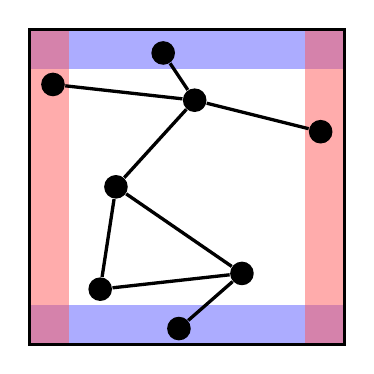
\begin{tikzpicture}[
            node/.style={circle, inner sep=0pt, fill=black, minimum size=3mm}
        ]
        \fill[blue!65, fill opacity=0.5] (0,0) rectangle (4, 0.5);
        \fill[blue!65, fill opacity=0.5] (0,3.5) rectangle (4, 4);
        \fill[red!65, fill opacity=0.5] (0,0) rectangle (0.5, 4);
        \fill[red!65, fill opacity=0.5] (3.5,0) rectangle (4, 4);
        \draw[black, very thick] (0,0) rectangle (4,4);
        \node[node] at (0.3, 3.3) (n1) {};
        \node[node] at (1.1, 2.0) (n2) {};
        \node[node] at (0.9, 0.7) (n3) {};
        \node[node] at (2.7, 0.9) (n4) {};
        \node[node] at (2.1, 3.1) (n5) {};
        \node[node] at (3.7, 2.7) (n6) {};
        \node[node] at (1.7, 3.7) (n7) {};
        \node[node] at (1.9, 0.2) (n8) {};
        \draw[very thick]  (n1) -- (n5);
        \draw[very thick]  (n5) -- (n2);
        \draw[very thick]  (n5) -- (n6);
        \draw[very thick]  (n2) -- (n4);
        \draw[very thick]  (n3) -- (n4);
        \draw[very thick]  (n2) -- (n3);
        \draw[very thick]  (n5) -- (n7);
        \draw[very thick]  (n8) -- (n4);
        \end{tikzpicture}
        \caption{non-percolating graph}
    \end{subfigure}
    %\hfill
    \begin{subfigure}[t]{0.55\textwidth}
        \centering
        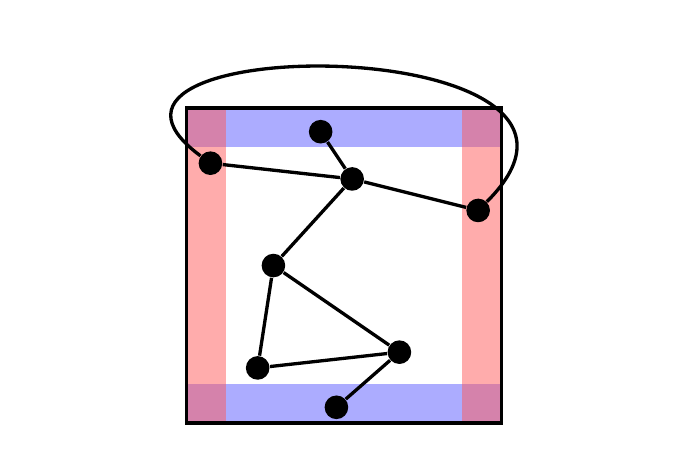
\begin{tikzpicture}[
            node/.style={circle, inner sep=0pt, fill=black, minimum size=3mm}
        ]
        \fill[blue!65, fill opacity=0.5] (0,0) rectangle (4, 0.5);
        \fill[blue!65, fill opacity=0.5] (0,3.5) rectangle (4, 4);
        \fill[red!65, fill opacity=0.5] (0,0) rectangle (0.5, 4);
        \fill[red!65, fill opacity=0.5] (3.5,0) rectangle (4, 4);
        \draw[black, very thick] (0,0) rectangle (4,4);
        \node[node] at (0.3, 3.3) (n1) {};
        \node[node] at (1.1, 2.0) (n2) {};
        \node[node] at (0.9, 0.7) (n3) {};
        \node[node] at (2.7, 0.9) (n4) {};
        \node[node] at (2.1, 3.1) (n5) {};
        \node[node] at (3.7, 2.7) (n6) {};
        \node[node] at (1.7, 3.7) (n7) {};
        \node[node] at (1.9, 0.2) (n8) {};
        \draw[very thick]  (n1) -- (n5);
        \draw[very thick]  (n5) -- (n2);
        \draw[very thick]  (n5) -- (n6);
        \draw[very thick]  (n2) -- (n4);
        \draw[very thick]  (n3) -- (n4);
        \draw[very thick]  (n2) -- (n3);
        \draw[very thick]  (n5) -- (n7);
        \draw[very thick]  (n8) -- (n4);
        \draw[very thick]  (n1) .. controls (-2,5) and (6,5) .. (n6);
        \end{tikzpicture}
        \caption{percolating graph}
    \end{subfigure}
    
    \caption{Illustration of percolating and non-percolating graphs.}
    \label{fig:percolation_example}
\end{figure}